\chapter{Vector differential equations and second-order circuits}

\section{Guess-and-check for RC filter with cosine input}
Last lecture we derived the folowing equation modeling the input-output properties of an amp: (where \(R\) is set by a potentiometer)
\begin{align}
  \dod{}{t} v_\text{out}(t)
  &= -\frac{1}{RC} v_\text{out}(t) + \frac{1}{RC} v_\text{in}(t);
  \quad \left.v_\text{out} \right|_{t_0} = V
  \intertext{
  In this section we will try to determine the result in \(v_\text{out}\) when \(v_\text{in}\) has the following sinusoidal form:
  }
  v_\text{in}(t)
  &= V_\text{in} \cos\del{\omega t}
  \intertext{This defines a sinusoid with amplitude \(V_\text{in}\) and a frequency of \(\omega\), which is angular frequency, in \(\unit{rad}/\unit{s}\).
  Angular frequency is related to cycles/second by \(\omega = 2\pi f\), where \(f\) is in units of \(\unit{Hz}\).}
  \intertext{
  We can solve for \(v_\text{out}\) by guessing that the particular solution----the summand that corresponds to \(v_\text{in}\)---has the form \(A\cos\del{\omega t + \phi}\).
  The second summand of \(v_\text{out}\) is the homogeneous solution, which corresponds to the initial condition.
  It has the form \(B e^{-\frac{1}{RC}(t - t_0)}\).
  }
  v_\text{out}(t)
  &= A \cos\del{\omega t + \phi}
  + B e^{-\frac{1}{RC} (t - t_0)}\label{eq:RC-cosine-solution}
  \intertext{Substitution into the differential equation and initial conditions result in the following constants:}
  A &= \frac{V_\text{in}}{\sqrt{\omega^2\del{RC}^2 + 1}}\\
  \phi &= -\tan^{-1}(\omega RC) \\
  B &= \left.v_\text{out}\right|_{t_0} - A \cos(\omega t_0 + \phi)
\end{align}

\section{Second-order filter with two capacitors}
\begin{figure}
  \centering
  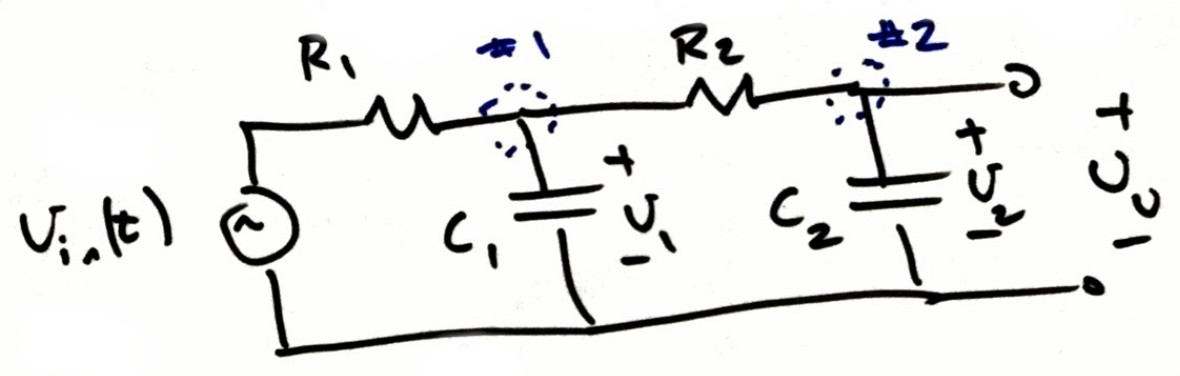
\includegraphics[width=1\linewidth]{figures/5/RCRC}
  \caption{Filter with two resistors and two capacitors.}
  \label{figure:lec5-RCRC}
\end{figure}
Perhaps a ``better'' filter could be constructed by using two capacitors and two resistors instead of just one.
\autoref{figure:lec5-RCRC} depicts the proposed circuit, which is a ``second-order circuit'' or ``second-order'' filter,
with values \(C_1 = C_2 = 1\unit{\(\mu\)F}\), \(R_1 = \frac{1}{3}\unit{M\(\Omega\)}\), and \(R_2 = \frac{1}{2}\unit{M\(\Omega\)}\).
KCL at the two dotted-circled upper nodes yields:
\begin{align}
  C_1 \dod{}{t} v_1 + \frac{v_1 - v_\text{in}(t)}{R_1} + \frac{v_1 - v_2}{R_2} &= 0\\
  C_2 \dod{}{t} v_2 + \frac{v_2 - v_1}{R_2} &= 0
\end{align}
In order to view this system of differential equations in state-space form, we will isolate derivatives on the LHS and emphasize that the RHS consists of linear combinations of \(v_1\), \(v_2\), and \(v_\text{in}(t)\):
\begin{align}
  \dod{}{t}v_1
  &= -v_1 \del{\del{\frac{1}{R_1} + \frac{1}{R_2}} \frac{1}{C_1}}
  + v_2 \del{\frac{ 1} {R_2C_1}} + v_\text{in}(t) \del{ \frac {1 }{R_1 C_1}}
  \\
  \dod{}{t} v_2
  &= \phantom{-}v_1 \del{\frac1 {R_2 C_2}} - v_2 \del{\frac 1 {R_2 C_2}}
  \intertext{
  Written in matrix-vector form with physical parameters substituted,
  }
  \dod{}{t}
  \begin{bmatrix}
    v_1\\v_2
  \end{bmatrix}
  &=
  \begin{bmatrix}
    -5 & \phantom{-}2\\
    \phantom{-}2 & -2
  \end{bmatrix}
  \begin{bmatrix}
    v_1\\v_2
  \end{bmatrix}
  % TODO use units
  +
  \begin{bmatrix}
    3\\0
  \end{bmatrix}
  v_\text{in}(t)
  \label{eq:lec5-RCRC-numerical}
\end{align}

\section{General state-space linear ODEs}
Generally, a system of linear differential equations similar to the one derived above has the following form:
\begin{align}
  \dod{}{t} \vec{x}
  &= A \vec{x} + \vec{b} u(t),
\end{align}
where \(\vec{x}\) is a vector and \(A\) is a \(2\times2\) matrix.

Suppose that \(A\) has an eigenvector \(\vec{v}\) for an eigenvalue \(\lambda\).
We propose the following solution to the homogeneous problem \(\od{}{t} \vec{x} = A \vec{x}\):
\begin{align}
  \vec{x} (t) = \vec{v} e^{\lambda t}
  \intertext{and verify that ``\(\od{}{t} \vec{x}\)'' and ``\(A \vec{x}\)'' for this candidate solution are equal:}
  \dod{}{t} \del{\vec{v} e^{\lambda t}}
  &= \lambda \vec{v} e^{\lambda t}\\
  A \del{\vec{v} e^{\lambda t}}
  &= \lambda \vec{v} e^{\lambda t}
\end{align}

\subsection{Detour: diagonalization of \(A\)}
Let's additionally assume that \(A\) has two linearly independent eigenvectors:
\begin{align}
  A \vec{v}_1 &= \lambda_1 \vec{v}_1 \\
  A \vec{v}_2 &= \lambda_2 \vec{v}_2
  \intertext{
  These two relationships can be expressed simultaneously using matrices that consolidate the eigenvectors (side by side) and eigenvalues (on a diagonal):
  }
  A
  \begin{bmatrix}
    \vec{v}_1 & \vec{v}_2
  \end{bmatrix}
  &=
  \begin{bmatrix}
    \vec{v}_1 & \vec{v}_2
  \end{bmatrix}
  \begin{bmatrix}
    \lambda_1 & 0 \\
    0 & \lambda _2
  \end{bmatrix}
  \intertext{Calling the former two matrices \(V\) and the latter \(\Lambda\),}
  AV &= V\Lambda
  \intertext{Because we chose two linearly independent eigenvectors to constitute \(V\), \(V\) is invertible.
  Stating \(A\) in terms of its eigenvectors and eigenvalues is called the \emph{eigenvector-eigenvalue decomposition} of \(A\):}
  A &= V \Lambda V^{-1}
\end{align}

\subsection{Second-order homogeneous solution from modes}
Generally, \(\vec{x}(0)\) will be a linear combination of \(\vec{v}_1\) and \(\vec{v}_2\):
\begin{align}
  \vec{x}(0)
  &= \tilde{x}_1(0) \vec{v}_1 + \tilde{x}_2(0) \vec{v}_2
  \label{eq:lec5-modal-decomp-IC}
  \intertext{These coefficients can be solved by inverting \(V\):}
  \begin{bmatrix}
    \tilde{x}_1 (0)\\
    \tilde{x}_2 (0)
  \end{bmatrix}
  &= V^{-1} \vec{x}(0)
  \intertext{We can build a homogeneous solution for \(\vec{x}(t)\) by superposing one-dimensional solutions in each eigenvector's respective direction:}
  \vec{x}(t)
  &= \vec{v}_1 e^{\lambda_1 t} \tilde{x}_1 (0)
  + \vec{v}_2 e^{\lambda_2 t} \tilde{x}_2 (0)\\
  &= V
  \begin{bmatrix}
    e^{\lambda_1 t} & 0\\
    0 & e^{\lambda_2 t}
  \end{bmatrix}
  \begin{bmatrix}
    \tilde{x}_1(0)\\
    \tilde{x}_2(0)
  \end{bmatrix}
  \intertext{To verify the initial condition, we can observe that the diagonal matrix of exponentials becomes an identity matrix at time \(0\):}
  \vec{x}(0) &=
  \begin{bmatrix}
    \vec{v}_1 & \vec{v}_2
  \end{bmatrix}
  \begin{bmatrix}
    1 & 0\\
    0 &1
  \end{bmatrix}
  \begin{bmatrix}
    \tilde{x}_1(0)\\
    \tilde{x}_2(0)
  \end{bmatrix},
\end{align}
which is true by construction (\autoref{eq:lec5-modal-decomp-IC}).

\subsection{Modal decomposition}
\begin{figure}
  \centering
  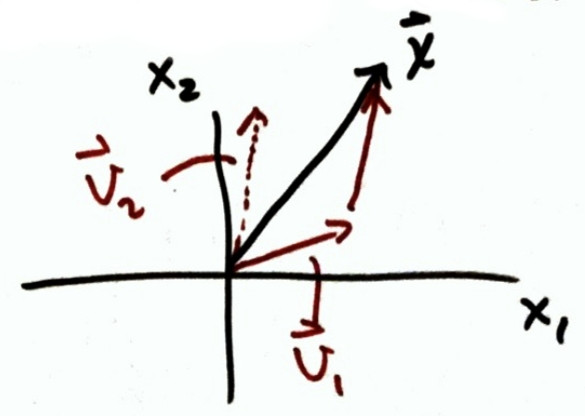
\includegraphics[width=0.5\linewidth]{figures/5/modal-synthesis}
  \caption{Decomposition of \(\vec{x}\) along eigenbasis directions \(\vec{v}_1\) and \(\vec{v}_2\).}
  \label{figure:lec5-modal-synthesis}
\end{figure}
In the previous section, we wrote \(\vec{x}(0)\) in eigenbasis-aligned coordinates \(\tilde{x}_1(0)\) and \(\tilde{x}_2(0)\).
In this section, we will follow \(\tilde{x}_1\) and \(\tilde{x}_2\) as functions of \(t\).
Recall that the eigenbasis-aligned coordinates are defined as follows:
\begin{align}
  \vec{x} &=
  \begin{bmatrix}
    \vec{v}_1 & \vec{v}_2
  \end{bmatrix}
  \begin{bmatrix}
    \tilde{x}_1 \\ \tilde{x}_2
  \end{bmatrix}
  = V \vec{\tilde x}.
  \intertext{In reverse,}
  \vec{\tilde x}
  &= V^{-1} \vec{x}.
  \intertext{We can use the Chain Rule to obtain a differential equation for \(\vec{\tilde x}\):}
  \dod{}{t} \vec{\tilde x}
  &= V^{-1} \dod{}{t} x\\
  &= V^{-1} \del{A \vec{x} + \vec{b} u}\\
  &= V^{-1} A V \vec{\tilde x} + V^{-1} \vec{b} u \\
  &=
  \begin{bmatrix}
    \lambda_1 & 0 \\
    0 & \lambda_2
  \end{bmatrix} \vec{\tilde x}
  + \vec{\tilde b} u, \quad \vec{\tilde b} = V^{-1} b
\end{align}
This vector differential equation is effectively scalar in each variable, in which scalar techniques can be applied separately.
The separation of \(x\) into its eigenbasis-aligned components is called \emph{modal decomposition};
\( \vec v_1 e^{\lambda_1 t}\) and
\( \vec v_2 e^{\lambda_2 t}\) are the two \emph{modes} of this system.
